\subsection{More on Semi-Cooper Problem}
This can be put into a specific potential. $V_{\vk,\vk'}=V_0w_\vk{}w_{\vk'}$ where $w_\vk=1$ for $k<\bar{k}$ and 0 otherwise. This very specific potential has one bound state solution for certain $V_0$.  

\begin{equation*}
-\frac{\hbar^2}{m}\frac{d^2}{dr^2}\chi+V\chi=E\chi
\end{equation*}
\begin{equation*}
\frac{\hbar^2}{m}k^2\chi_k+\sum_{k'}V_{k,k'}\chi_{k'}=E\chi_k
\end{equation*}
\begin{equation*}
\frac{\hbar^2}{m}k^2\chi_k+V_0\sum_{k'<\bar{k}}\chi_{k'}=E\chi_k
\end{equation*}
We are seeking a bound-state solution for $E<0$.  Introduce $|E|\equiv\frac{\hbar^2}{m}k_0^2$, and sum the lhs over $k<\bar{k}$, we have 
\[
1=V_0\sum\frac{w_k}{-\epsilon_k+E}=\abs{V_0}\frac{m}{\hbar^2}\sum\frac{w_k}{k^2+k_0^2}
\]
introduce 
\begin{equation}
A=\frac{mV}{2\pi^2\hbar^2}\abs{V_0}
\end{equation}
where $V$ is the volume. And we have equation
\begin{equation}\label{eq:boundCooper}
\nth{A}=\int^{\bar{k}}_0\frac{k^2}{k_0^2+k^2}dk=\bar{k}-k_0\arctan\frac{\bar{k}}{k_0}
\end{equation}
and we have 
\begin{equation}\label{eq:arctan}
\bar{k}-\nth{A}=k_0\arctan\frac{\bar{k}}{k_0}
\end{equation}

A rough analysis tells us that introduce the open-channel background is somewhat equivalent to decrese the strength of interaction $\abs{V_0}$; this means decreasing of $A$ as well as the lhs of eq. \eqref{eq:arctan}. So we expect the decrease of $k_0$ as in fig. \ref{fig:arctan}, so smaller binding energy $|E|$ and larger close-channel bound-state. 
\begin{figure}[htb]
	\centering
		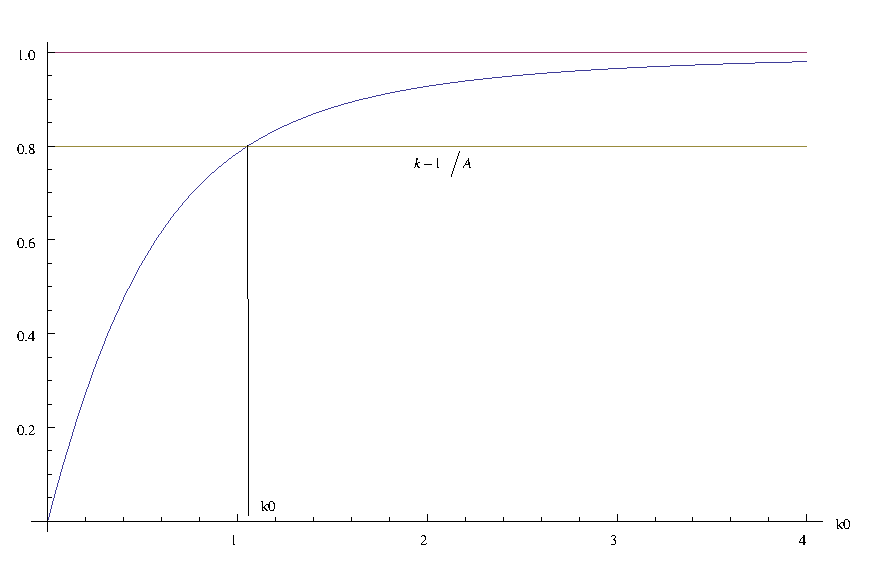
\includegraphics[width=.50\textwidth]{image/arctan.eps}
	\caption{Plot of $k_0\arctan\frac{\bar{k}}{k_0}$\label{fig:arctan}}
\end{figure}
This seems to indicate that less weight in the center for coupling to open-channel.  

Particularly, for the simple Fermi sea background, the integration in eq. \eqref{eq:boundCooper} starts from $k_F$ instead of 0.  
\[
\nth{A}=\int^{\bar{k}}_{k_F}\frac{k^2}{k_0^2+k^2}dk=\bar{k}-k_F-k_0\br{\arctan\frac{\bar{k}}{k_0}-\arctan\frac{k_F}{k_0}}
\]
If we take the fact that the bound-state in close-channel is much smaller than the inter-particle space, we can expand the last term and keep only the lowest two term. 
\begin{equation}
\bar{k}-\nth{A}=k_0\arctan\frac{\bar{k}}{k_0}+\nth{3}k_F(\frac{k_F}{k_0})^2
\end{equation}
And we find the correction on $k_0$ is
\footnote{
\[
\br{k_0\arctan\frac{\bar{k}}{k_0}}'=\arctan\frac{\bar{k}}{k_0}--\frac{k_0\bar{k}}{\bar{k}^2+k_0^2}
\]
}
\begin{equation}
\delta{}k_0=-\frac{\nth{3}k_F}{\arctan\frac{\bar{k}}{k_0}-\frac{k_0\bar{k}}{\bar{k}^2+k_0^2}}(\frac{k_F}{k_0})^2
\end{equation}
If $\bar{k}\gg{}k_0$, $\arctan\frac{\bar{k}}{k_0}\simeq\frac{\pi}2$ and 
\begin{equation}
\delta{}k_0=-\frac{2}{3\pi}{k_F}(\frac{k_F}{k_0})^2
\end{equation}
and 
\begin{equation}\label{eq:BcsShiftE}
\delta{|E|}=-\frac{8}{3\pi}{\epsilon_F}(\frac{k_F}{k_0})
\end{equation}


In the extreme-BEC side, the open-channel background has $n_k\sim{}na_s^3$ (eq. 2.38 in\cite{ZhangThesis}), where $n$ is the density, $a_s$ is the s-wave scattering length/size of \emph{open-channel} molecules.  This add a factor $(1-n_k)$ (or $(1-n_k)^2$?)  into integral of eq. \eqref{eq:boundCooper}.  And similarly
\begin{equation}
\delta{}k_0=-\frac{\nth{A}}{\arctan\frac{\bar{k}}{k_0}-\frac{k_0\bar{k}}{\bar{k}^2+k_0^2}}n_k
\end{equation}
If $\bar{k}\gg{}k_0$ and 
\begin{equation}
\delta{}k_0=-\frac{2}{\pi}\nth{A}na_s^3
\end{equation}
and 
\begin{equation}\label{eq:BecShiftE}
\delta{|E|}=-\frac{4\hbar^2}{\pi{}m}k_0\nth{A}na_s^3=-\frac{4\hbar^2}{\pi{}m}k_0(\bar{k}-k_0\arctan\frac{\bar{k}}{k_0})na_s^3
\end{equation}
This shift depends on the specific form of the pentential; while at the very BCS side, the shift of binding energy, eq. \eqref{eq:BcsShiftE}, is independent of the form of the pontential. It seems that it is not necessarily to know simply the binding energy/s-wave scattering length of the close-channel bound state in this problem.  

(\emph{This part about BEC limit is wrong as discussed in below.})


\subsection{Additional note from 2009.12.17\label{subsec:additionalSemiCooper}}
For large molecule/small binding energy/small $k_0$, we have $\bar{k}-\nth{A}\approx\frac{\pi}{2}k_0-\frac{k_0^2}{\bar{k}}$.   And the correction in the lowest order (ignoring the second term) is $\frac{\pi}{2}\delta{}k_0$ for any extra terms. 

So for a background of open-channel $f(k)$, from eq. (\ref{eq:boundCooper}), we find that 
\begin{equation*}
\nth{A}=\int^{\bar{k}}_0\frac{k^2}{k_0^2+k^2}(1-f(\vk))dk=\bar{k}-k_0\arctan\frac{\bar{k}}{k_0}-\int^{\bar{k}}_0\frac{k^2}{k_0^2+k^2}f(k)dk
\end{equation*}
And in the lowset order 
\begin{equation*}
0=-\left.\frac{d(k_0\arctan\frac{\bar{k}}{k_0})}{dk_0}\right|_{k_0=k^{(0)}_0}\delta{}k_0-\int^{\bar{k}}_0\frac{k^2}{k_0^2+k^2}f(k)dk
\end{equation*}
When binding energy/$k_0$ is small, the derivative is just $\frac{\pi}2$ and 
\begin{equation}
\delta{}k_0=-\frac{2}{\pi}\int^{\bar{k}}_0\frac{k^2}{k_0^2+k^2}f(k)dk
\end{equation}
The rhs only relates to $k_0$ if $f(k)$ falls off earlier than $\bar{k}$ which is the case we are interesting as the open-channel feature is always larger than the close-channel bound-state in real space.  Particularly in BEC limit, as open-channel molecule (size $a_s$) is larger  than close-channel molecule ($1/k_0$), and we can assume a very simple form of $f(k)=na_s^3$ where $k$ is in $(0,1/a_s)$, otheerwise $f(k)=0$.  Also taking considering the fact that $1/a_s\ll{}k_0\ll,\bar{k}$ we can find the result is
\begin{equation}
\delta{}k_0=-\frac{2}{\pi}{k_0}\int^{1/a_s}_0\frac{k^2}{k_0^2+k^2}na_s^3dk\approx-\frac{2}{\pi}\int^{1/a_s}_0\frac{k^2}{k_0^2}na_s^3dk=-\frac{2}{3\pi}\frac{n}{k^2_0}
\end{equation}
And the correction of binding energy is
\begin{equation}
\delta{}|E|=2\hm{}k_0\delta{}k_0=-\frac{4}{3\pi}|E|\frac{n}{k_0^3}
\end{equation}
where the last term can be seen as the ration between  the size of  bound-state molecules and interparticle distance. 